\documentclass{standalone}
\usepackage{tikz}
\usepackage{ctex,siunitx,ninecolors}
\setCJKmainfont{Noto Serif CJK SC}
\usepackage{tkz-euclide}
\usepackage{amsmath}
\usetikzlibrary{patterns, calc}
\usetikzlibrary {decorations.pathmorphing, decorations.pathreplacing, decorations.shapes}
\begin{document}
\small
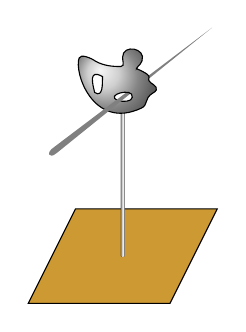
\begin{tikzpicture}[>=latex,scale=1.2]
  \draw[fill=brown!80!yellow](-1,-0.5)--(0.5,-0.5)--(1,0.5)--(-0.5,0.5)--cycle;
  \fill[left color=gray,right color=gray,middle color=white](-0.02,0)arc(180:360:0.02 and 0.01)--(0.02,1.6)--(-0.02,1.6)--cycle;
  \fill[gray](0.945,2.418)--(-0.0062,1.6985)--(0.0224,1.6730)--cycle;
  \fill[ball color=lightgray,draw=black]( 0.145,1.985)..controls( 0.373,1.885)and( 0.222,1.897)..
  ( 0.299,1.833)..controls( 0.330,1.812)and( 0.405,1.773)..
  ( 0.316,1.724)..controls( 0.222,1.667)and( 0.275,1.600)..
  ( 0.194,1.565)..controls(-0.315,1.329)and(-0.519,1.952)..
  (-0.461,2.097)..controls(-0.445,2.142)and(-0.343,2.101)..
  (-0.289,2.064)..controls(-0.198,2.011)and(-0.094,2.008)..
  (-0.046,2.007)..controls(-0.035,2.009)and(-0.005,1.999)..
  ( 0.003,2.020)..controls( 0.012,2.049)and( 0.000,2.050)..
  (-0.001,2.104)..controls(-0.002,2.249)and( 0.252,2.203)..
  ( 0.204,2.067)..controls( 0.179,2.011)and( 0.174,2.031)..cycle
  (-0.214,1.901)..controls(-0.369,1.987)and(-0.316,1.814)..
  (-0.297,1.732)..controls(-0.205,1.671)and(-0.216,1.829)..cycle
  ( 0.101,1.681)..controls( 0.121,1.794)and(-0.209,1.704)..
  (-0.044,1.646)..controls( 0.007,1.631)and( 0.097,1.635)..cycle;
  \fill[gray](-0.0062,1.6985)--(-0.729,1.152)..controls(-0.813,1.099)and(-0.786,1.019)..(-0.699,1.091)--(0.0224,1.6730);
\end{tikzpicture}
\end{document}